\documentclass[../../main.tex]{subfiles}

\begin{document}
For ease of reference, we repeat the ``RSA handshake'' diagram in
Figure~\ref{fig:rsa-handshake-repeat}. The long-term private key, in
this scenario, is required for decrypting \premaster. As such,
~\premaster~must be passed to the \textit{enclave program} for
decryption. However, an interface that accepts ~\premaster, and
returns \texttt{PremasterSecret} unencrypted compromises the long-term
private key. Such an interface is an \textit{oracle} for the long-term
private key, providing an adversary who exploits the untrusted
component the ability to decrypt any cipher-text by invoking this
interface.

\begin{figure}[H]
  \centering
  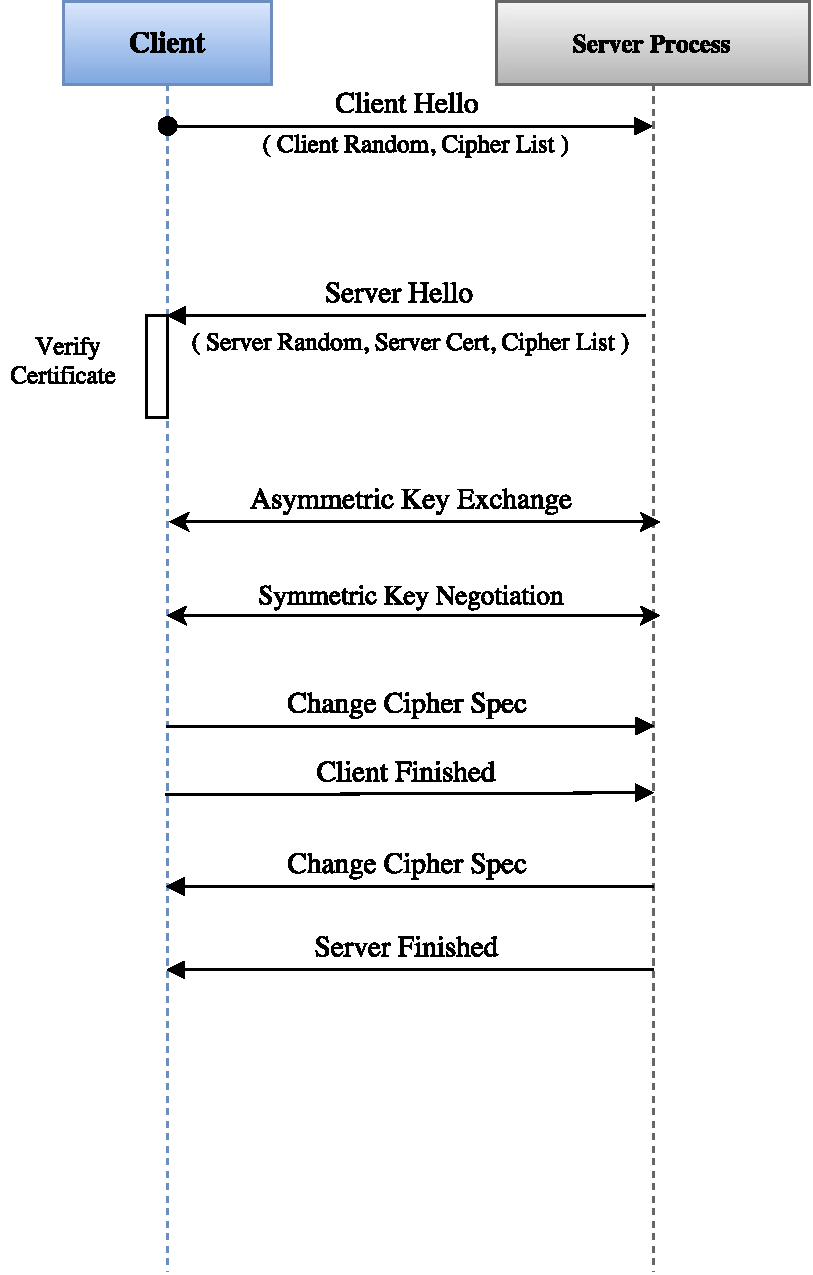
\includegraphics[scale=0.4]{images/rsa-handshake-pristine.pdf}
  \caption{``RSA handshake''}
  \label{fig:rsa-handshake-repeat}
\end{figure}

Reviewing the steps for session key generation, detailed in
Section~\ref{sec:ssloverview}, the decrypted \texttt{PremasterSecret},
along with \crandom~ and \srandom, is passed to a PRF to compute
\texttt{MasterSecret}. Output of a PRF is \textit{preimage resistant},
meaning that the output cannot be mapped back to the input; hence, we
may choose to offer an interface that accepts \crandom, \srandom, and
\premaster, and returns \texttt{MasterSecret}. However, such an
interface allows an adversary to \textit{influence} the generation of
\texttt{MasterSecret}. To be precise, it allows an adversary to
generate the \texttt{MasterSecret} for any eavesdropped session
(\srandom~and \crandom~are both sent in the clear, and the interface
takes \premaster, all of these are easily captured by a passive
eavesdropper).

Instead, we offer the same interface proposed in the Wedge paper, and
detailed in Section~\ref{sec:polp}. This interface accepts \crandom~
and \premaster, both provided by the client, and returns
\texttt{MasterSecret}. \srandom~is generated by the \textit{enclave
  program} and used in computing \texttt{MasterSecret}. By designing
the interface in this manner, we retain the freshness property
discussed earlier. Consequently, an adversary who exploits the
untrusted component is no longer capable of influencing the
\texttt{MasterSecret} generation routine, because one of its
parameters, \srandom, is computed by the \textit{enclave program}.
The resulting design is illustrated in Figure~\ref{fig:rsa-enc}.

\begin{figure}[H]
  \centering
  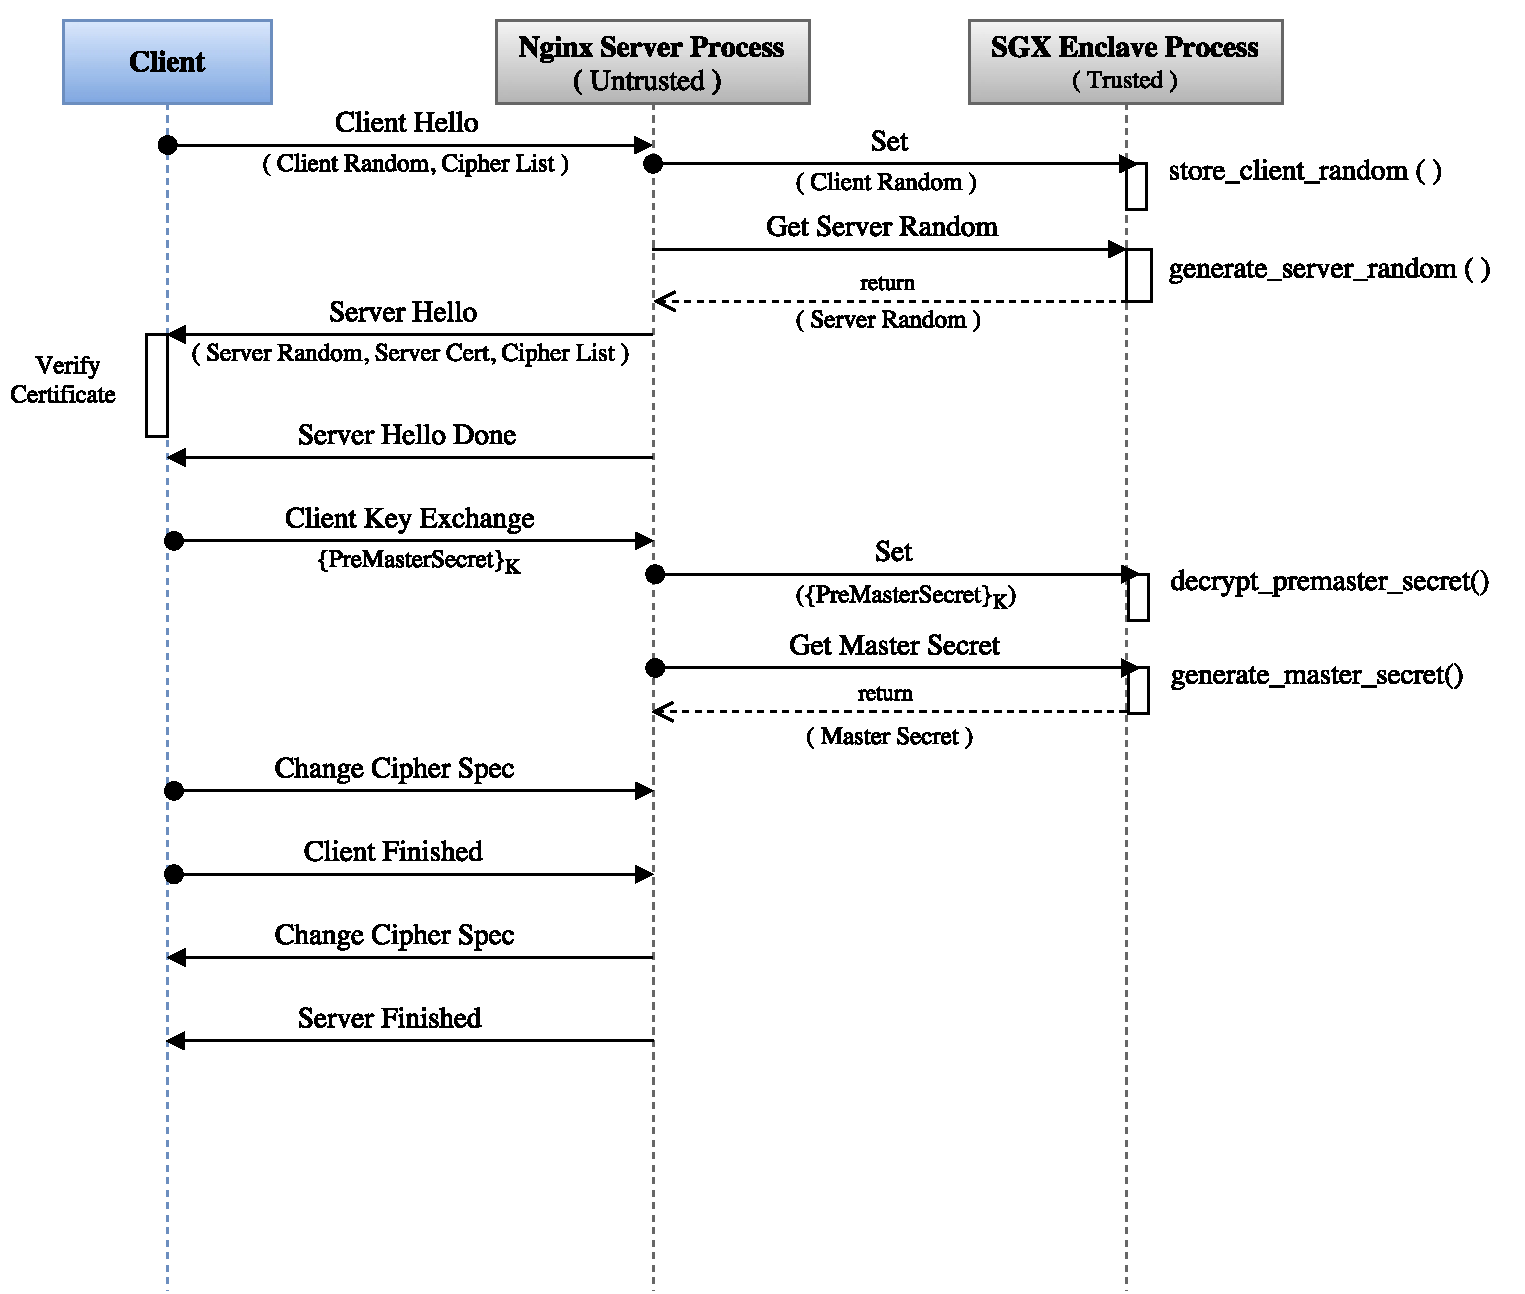
\includegraphics[scale=0.35]{images/RSA-SGX-Handshake.pdf}
  \caption[``RSA handshake'' and enclave]{``RSA handshake'' with
    private key in an SGX enclave}
  \label{fig:rsa-enc}
\end{figure}

For clarification, we explain the ``RSA handshake's'' execution within
the context of our design. The handshake begins with the client
connecting to the server by sending a \texttt{ClientHello} message.
The \crandom~ value contained in this message is passed to the
enclave, preparing for \texttt{MasterSecret}'s derivation. After
successfully feeding the enclave with \crandom, the untrusted
component sends a command to the \textit{enclave program}, requesting
the generation of \srandom. Upon receiving ~\srandom~from the
\textit{enclave program}, the server replies to the client with a
\texttt{ServerHello} message, followed by a \texttt{ServerDone}
message. \texttt{ServerDone} informs the client that the server is
ready to proceed to the key negotiation phase. The client responds with a
\texttt{ClientKeyExchange} message, containing \premaster, where
\texttt{K} is the server's public key. The server forwards
\premaster~to the \textit{enclave program}. The code running within
the enclave uses the provisioned long-term private key to decrypt
\premaster. The now-decrypted \texttt{PremasterSecret}, along with the
pre-negotiated \crandom~and \srandom~values are input to the
aforementioned PRF, outputting \texttt{MasterSecret}. The remainder of
the handshake continues without any more interactions with the
\textit{enclave program} \footnote{Actually, there is one more
  interaction with the enclave upon successful termination of an SSL
  handshake. This is mostly an implementation detail regarding SSL
  session management and Nginx's event-driven design and is not
  directly connected with the SSL/TLS protocol itself. We reason
  further about this requirement in Section
  \ref{sec:implementation}.}. %I am still figuring out where to place
                              %this, bear with me.

% Freshness of the generated session-key has been used in [WEDGE
% CITATION] to maintain the secrecy of an SSL/TLS private key in the
% face of a passive eavesdropper how can exploit the server
% application's network facing process. We use it to secure the
% private key against an adversary who can exploit the underlying
% operating system and/or a malicious cloud provider.
\end{document}
%%% Local Variables:
%%% mode: latex
%%% TeX-master: "../../main"
%%% End:
